% PACKAGES INCLUDED HERE 
% DO NOT NEED TO CHANGE
\documentclass[conference]{IEEEtran}
%\IEEEoverridecommandlockouts
% The preceding line is only needed to identify funding in the first footnote. If that is unneeded, please comment it out.
\usepackage{listings}
\usepackage{csquotes}
\usepackage{float}
\usepackage[caption=false]{subfig}
\usepackage{cite}
\usepackage{amsmath,amssymb,amsfonts}
\usepackage{algorithmic}
\usepackage{graphicx}
\usepackage{textcomp}
\usepackage{hyperref}
\usepackage{url}
\def\BibTeX{{\rm B\kern-.05em{\sc i\kern-.025em b}\kern-.08em
    T\kern-.1667em\lower.7ex\hbox{E}\kern-.125emX}}
\begin{document}

% TITLE GOES HERE

\title{Predicting Pseudo Random Values Using Convolutional Neural Networks\\}


% AUTHOR NAMES GOES HERE


\author{
\IEEEauthorblockN{Najib Ali}
\IEEEauthorblockA{\textit{Department of Computer Science}\\
\textit{Middle Tennessee State University}\\
Murfreesboro, Tennessee \\
email address}\\[0.4cm]  %<------- Extra vertical space
\IEEEauthorblockN{Matthew Hawks}
\IEEEauthorblockA{\textit{Department of Computer Science}\\
\textit{Middle Tennessee State University}\\
Murfreesboro, Tennessee \\
email address}
\and
\IEEEauthorblockN{Jacob Anderson}
\IEEEauthorblockA{\textit{Department of Computer Science}\\
\textit{Middle Tennessee State University}\\
Murfreesboro, Tennessee \\
email address}\\[0.4cm]  %<------- Extra vertical space
\IEEEauthorblockN{Ryan Hines}
\IEEEauthorblockA{\textit{Department of Computer Science}\\
\textit{Middle Tennessee State University}\\
Murfreesboro, Tennessee \\
email address}
\and
\IEEEauthorblockN{Spencer Arnold}
\IEEEauthorblockA{\textit{Department of Computer Science}\\
\textit{Middle Tennessee State University}\\
Murfreesboro, Tennessee \\
email address}\\[0.4cm]  %<------- Extra vertical space
\IEEEauthorblockN{Tae Kweon}
\IEEEauthorblockA{\textit{Department of Computer Science}\\
\textit{Middle Tennessee State University}\\
Murfreesboro, Tennessee \\
email address}
}

\maketitle

% ABSTRACT 

\begin{abstract}
This document is a model and instructions for \LaTeX.
This and the IEEEtran.cls file define the components of your paper [title, text, heads, etc.]. *CRITICAL: Do Not Use Symbols, Special Characters, Footnotes, 
or Math in Paper Title or Abstract.
This document is a model and instructions for \LaTeX.
This and the IEEEtran.cls file define the components of your paper [title, text, heads, etc.]. *CRITICAL: Do Not Use Symbols, Special Characters, Footnotes, 
or Math in Paper Title or Abstract.
This document is a model and instructions for \LaTeX.
This and the IEEEtran.cls file define the components of your paper [title, text, heads, etc.]. *CRITICAL: Do Not Use Symbols, Special Characters, Footnotes, 
or Math in Paper Title or Abstract.
This document is a model and instructions for \LaTeX.
This and the IEEEtran.cls file define the components of your paper [title, text, heads, etc.]. *CRITICAL: Do Not Use Symbols, Special Characters, Footnotes, 
or Math in Paper Title or Abstract.

\end{abstract}


% KEYWORDS

\begin{IEEEkeywords}
component, formatting, style, styling, insert
\end{IEEEkeywords}

% INTRODUCTION SECTION
\section{Introduction}

Start typing here \cite{b1}.

% BACKGROUND SECTION
\section{Background}

Start typing here \cite{b2}.

% METHODS SECTION
\section{Methods}
\subsection{Seeding Method}
We went with a seed generation method that allowed a way to introduce some minor level of entropy to avoid letting the neural network aimlessly swim through the entropy of a strong seed instead of gaining stochastic insight on the data from the PRNG. \newline
The seed generation method we chose derives from the concept of using the system time as an element for seed generation. The specific implementation we chose took inspiration from Microsoft's .NET system.datetime.ticks property. \cite{b1} We chose to single out this method due to its documentation and unqiue simplicity. System time is widely used as a parameter for modern seed generation methods. To put it more trivially: "a pseudo random number generator is a deterministic algorithm that, given an initial number (called seed), generates a sequence of numbers that adequately satisfies statistical randomness tests. Since the algorithm is deterministic, the algorithm will always generate the exact same sequence of numbers if it's initialized with the same seed. That's why system time (something that changes all the time) is usually used as the seed for random number generators." \cite{b2} \newline
According to the Microsoft documentation, "A single tick represents one hundred nanoseconds or one ten-millionth of a second. There are 10,000 ticks in a millisecond, or 10 million ticks in a second. The value of this property represents the number of 100-nanosecond intervals that have elapsed since 12:00:00 midnight, January 1, 0001 in the Gregorian calendar." \cite{b1}  \newline
We used a fairly similar Python port, explained below. \cite{b3}
\lstset{language=Python}
\begin{lstlisting}[breaklines=true]
def ticks(dt):
    return (dt-datetime(1,1,1)).total_seconds()*10000000
\end{lstlisting} 

Porting side effects include:
\begin{enumerate}
    \item UTC times are assumed.
    \item The resolution of the datetime object is given by datetime.resolution, which is datetime.timedelta(0, 0, 1) or microsecond resolution (1e-06 seconds). CSharp Ticks are purported to be 1e-07 seconds.
\end{enumerate}

Additional changes we made to our implementation:
\begin{enumerate}
    \item Changing start time from January 1, 0001 to January 1, 1970, which effectively reduced the length of the seed for experimental purposes.
    \item Slicing last 6 digits of the ticks result to acquire more digit variation for frequent invocation.
\end{enumerate}

This final method allows enough spread between frequently retreived ticks, where we are assuming reasonable pseudo-unpredictabililty. This serves as a simplistic but constantly changing control mechanism for being able to seed PRNGs and test experimental outcomes. While not the most cryptographically strong, we needed a way to have some controlled aspect of seed generation to feed into generators of varying cryptographic complexity (to have some baseline of comparison).\newline

The original idea was to feed each PRNG different seeds from the same seed generator; however, many PRNG algorithms impose strict seed requirements to pass tests of randomness. Out of the five PRNG methods we implemented, Lagged Fibonacci was the only one that had special seed requirements, so we created a separate seed generator based on the same fundamental ticks generation method, but modified to meet the restrictions. Other PRNGs not implemented in this research that impose seed restrictions include Wichmann-Hill (which accepts three different seeds) and Maximally Periodic Reciprocals (which requires a Sophie Prime), among others.\newline

You might ask: won't different seed generators introduce flaws or bias in the experiment? Well, it depends on what you are testing. In our case, we are strictly testing the "complexity" of the generator itself, so supplying a seed that is not blatantly predictable but also not unpredictable was sufficient. Our goal was to allow the charactaristics of the generator to be exposed, for we were cracking the "complexity" of the generation algorithm, not the complexity of an arbitrary seed.

\subsection{PRNG Implementations}
\subsection{Predictive Network}
NOTE THE Equation will have to be re-done and diagrams re-drawn to reflect our experiment.
The predictor is a convolutional neural network implementing the function ...
: $P(r_{split}) \mathbb{B}$ 7→B(7)wherersplitis  the  generator’s  output  vector  with  the  last  element  removed.The  last  element  is  used  as  the  corresponding  label  for  the  predictor’s  input.
\begin{figure}[H]
\centering
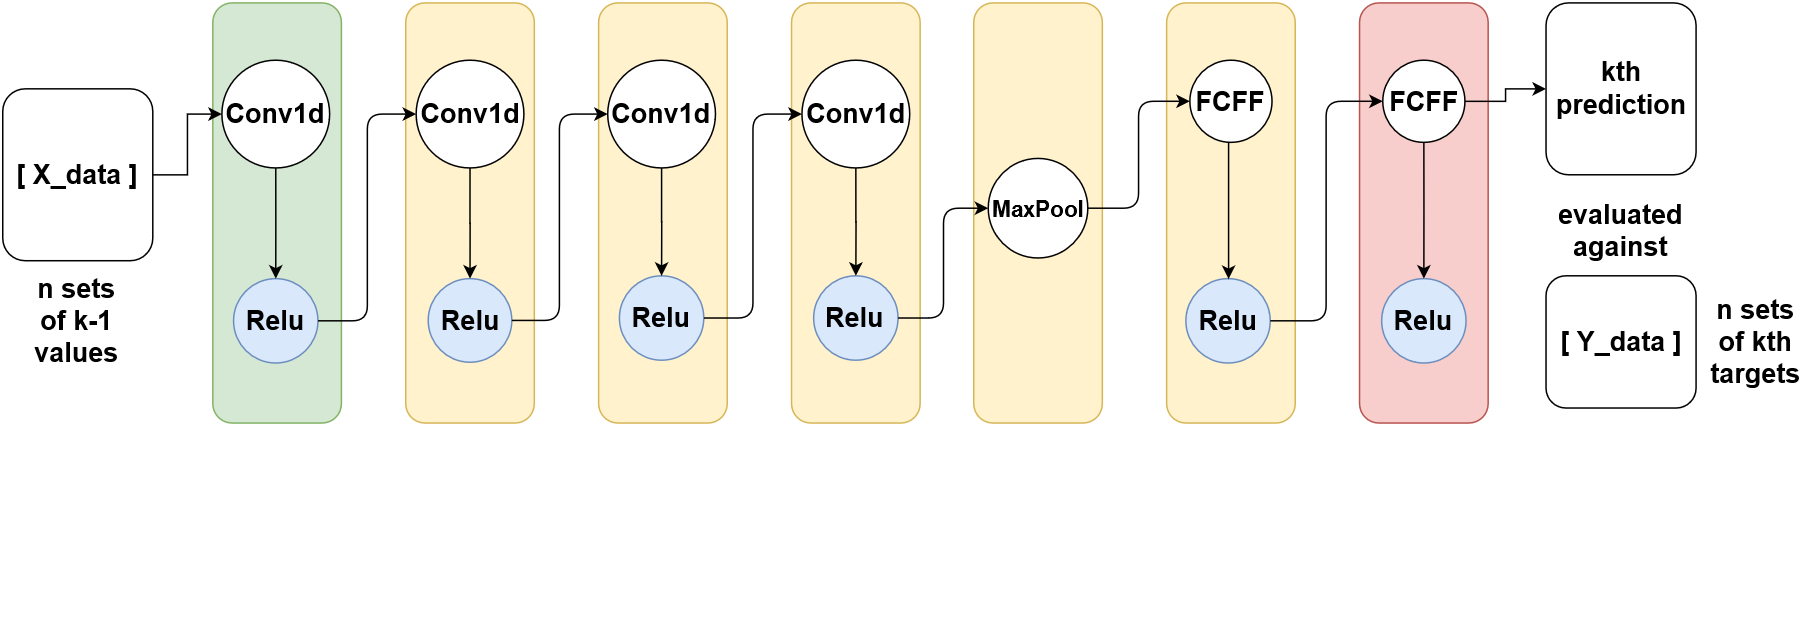
\includegraphics[width=1\linewidth]{./Images/PredictiveModel.png}
\caption{Predictive Model}
\label{fig:globfig}
\end{figure}

\subsection{Experimental Setup}
\begin{figure}[H]
\centering
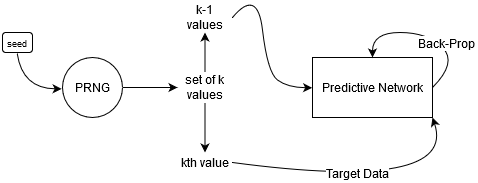
\includegraphics[width=1\linewidth]{./Images/SimpleModel.png}
\caption{Experiment Model}
\label{fig:globfig}
\end{figure}

\subsection{Experimental Setup}
\begin{figure}[H]
\centering
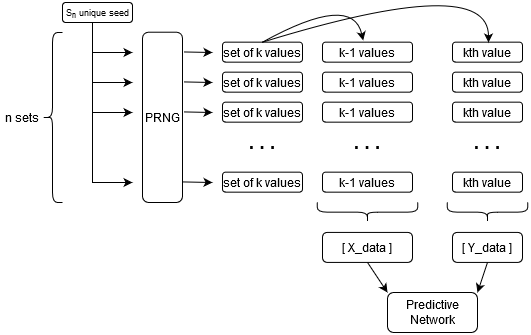
\includegraphics[width=1\linewidth]{./Images/GranularModel.png}
\caption{Experiment Model}
\label{fig:globfig}
\end{figure}


% RESULTS SECTION
\section{Results}

\begin{figure}[H]
\centering
\subfloat[Subfigure 1 list of figures text][Testing Regression Plot]{
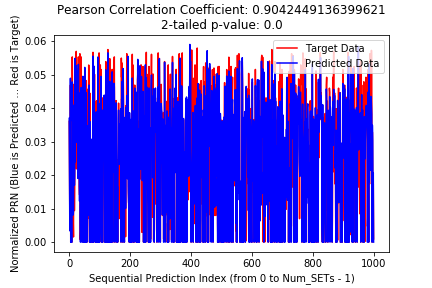
\includegraphics[width=0.4\linewidth]{./Images/Middle_Square_Reg.png}
\label{fig:subfig1}}
\qquad
\subfloat[Subfigure 2 list of figures text][Training Loss Plot]{
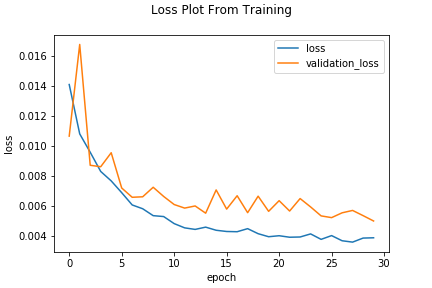
\includegraphics[width=0.4\linewidth]{./Images/Middle_Square_Loss.png}
\label{fig:subfig2}}
\caption{Middle Square Results}
\label{fig:globfig}
\end{figure}

\begin{figure}[H]
\centering
\subfloat[Subfigure 1 list of figures text][Testing Regression Plot]{
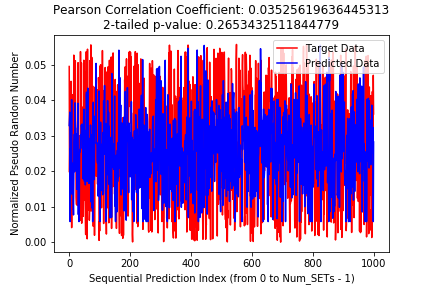
\includegraphics[width=0.4\linewidth]{./Images/Linear_Cong_Reg.png}
\label{fig:subfig1}}
\qquad
\subfloat[Subfigure 2 list of figures text][Training Loss Plot]{
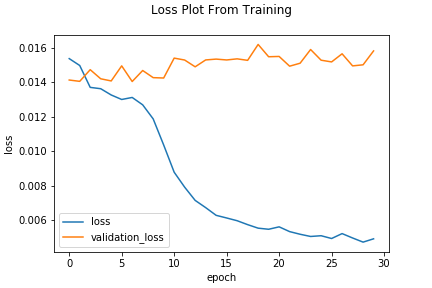
\includegraphics[width=0.4\linewidth]{./Images/Linear_Cong_Loss.png}
\label{fig:subfig2}}
\caption{Linear Congruential Results}
\label{fig:globfig}
\end{figure}

\begin{figure}[H]
\centering
\subfloat[Subfigure 1 list of figures text][Testing Regression Plot]{
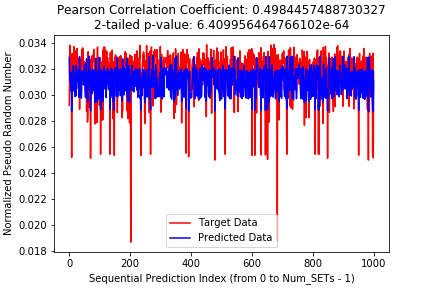
\includegraphics[width=0.4\linewidth]{./Images/Lagged_Fib_Reg.png}
\label{fig:subfig1}}
\qquad
\subfloat[Subfigure 2 list of figures text][Training Loss Plot]{
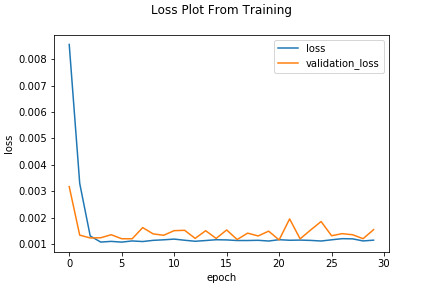
\includegraphics[width=0.4\linewidth]{./Images/Lagged_Fib_Loss.png}
\label{fig:subfig2}}
\caption{Lagged Fibonacci Results}
\label{fig:globfig}
\end{figure}

\begin{figure}[H]
\centering
\subfloat[Subfigure 1 list of figures text][Testing Regression Plot]{
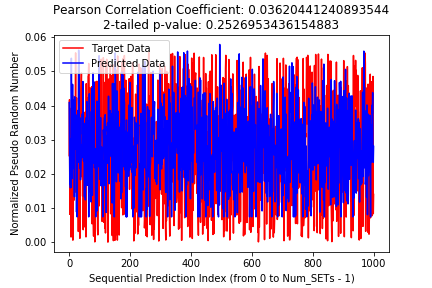
\includegraphics[width=0.4\linewidth]{./Images/Park_Miller_Reg.png}
\label{fig:subfig1}}
\qquad
\subfloat[Subfigure 2 list of figures text][Training Loss Plot]{
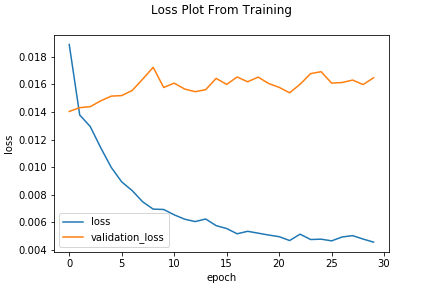
\includegraphics[width=0.4\linewidth]{./Images/Park_Miller_Loss.png}
\label{fig:subfig2}}
\caption{Park Miller Results}
\label{fig:globfig}
\end{figure}

\begin{figure}[H]
\centering
\subfloat[Subfigure 1 list of figures text][Testing Regression Plot]{
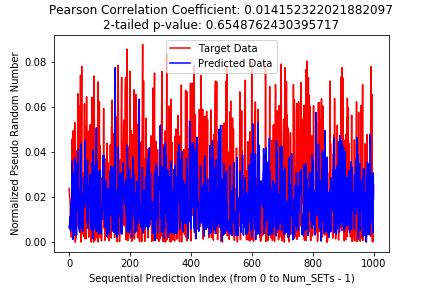
\includegraphics[width=0.4\linewidth]{./Images/Twister_Reg.png}
\label{fig:subfig1}}
\qquad
\subfloat[Subfigure 2 list of figures text][Training Loss Plot]{
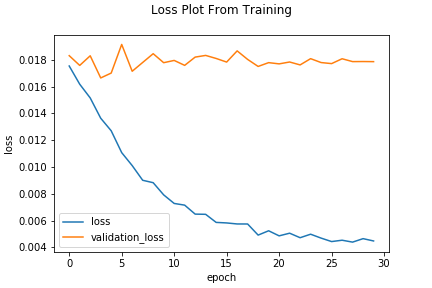
\includegraphics[width=0.4\linewidth]{./Images/Twister_Loss.png}
\label{fig:subfig2}}
\caption{Mersenne Twister Results}
\label{fig:globfig}
\end{figure}

% DISCUSSION SECTION
\section{Discussion}
Start typing here her is Start typing here her isStart typing here her isStart typing here her isStart typing here her isStart typing here her isStart typing here her isStart typing here her isStart typing here her isStart typing here her isStart typing here her isStart typing here her isStart typing here her isStart typing here her isStart typing here her isStart typing here her isStart typing here her isStart typing here her isStart typing here her isStart typing here her isStart typing here her isStart typing here her isStart typing here her isStart typing here her isStart typing here her isStart typing here her isStart typing here her isStart typing here her isStart typing here her isStart typing here her is

.. code:: ipython3

    % REFERENCES
    % THIS IS CREATED AUTOMATICALLY
    \bibliographystyle{IEEEtran}
    \bibliography{References} % change if another name is used for References file

\end{document}
